\documentclass[11pt]{standalone}
\usepackage{tikz, pgfplots,amsmath, amssymb, amsthm}   
\usepgfplotslibrary{groupplots}


\begin{document}


  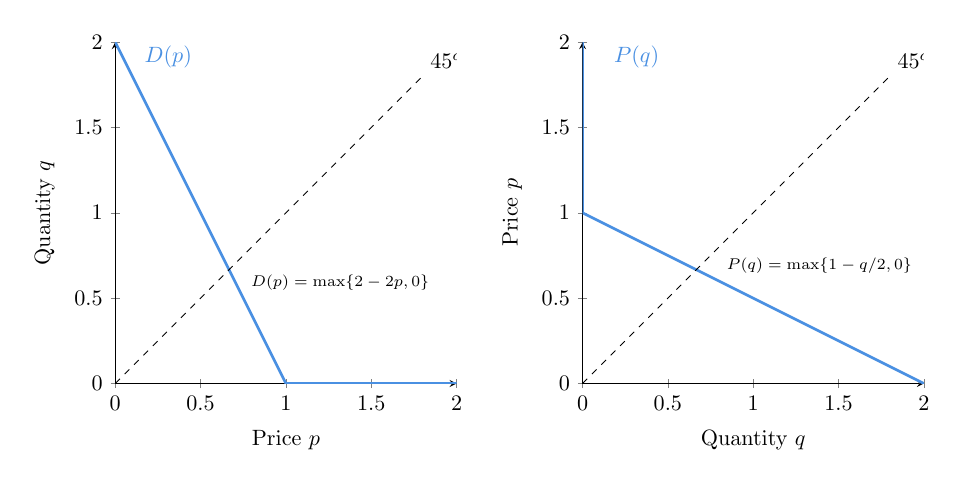
\begin{tikzpicture}[scale=.8]
    \begin{groupplot}[
      group style={group size=2 by 1, horizontal sep=2cm}, no markers,
      height=7cm, width=7cm,
      axis x line=bottom, axis y line=left,
      ymin=0, ymax=24,
      extra y ticks={23},  extra y tick labels={$\mathbf{E}\{R\}$},
    extra y tick style={major tick length=0mm, grid=none},
    scatter/classes={
      a={mark=o,draw=black, mark size = 3pt},
      b={mark=*, mark size = 3pt,draw=red, fill = red},
      c={mark=*, mark size = 3pt,draw=black, fill = black}
    }
]
% PLOT 1
\nextgroupplot[
   xlabel = Price $p$, ylabel = Quantity $q$,
  ymin=0, ymax=2, xmin=0, xmax=2,
  extra x ticks={3.5}, extra x tick labels={$P$},
  extra x tick style={major tick length=0mm, grid=none},
  extra y ticks={3.5}, extra y tick labels={$Q$},
  extra y tick style={major tick length=0mm,  grid=none},
]
    
\addplot[scatter,only marks, scatter src=explicit symbolic]
  coordinates {(20, 11) (12, 5) };

\node at (axis cs:12, 5) [anchor=south west] {A};
\node at (axis cs:20,11) [anchor=north west] {B};
\draw[color={rgb, 255:red,74;green,144;blue,226}, very thick] (axis cs:1,0) -- (axis cs:2,0) ;
\addplot[color={rgb, 255:red,74;green,144;blue,226}, very thick,  domain=0:3, samples=1000, variable=\t]({t},  {2-2*t} )  node[color={rgb, 255:red, 74; green, 144; blue, 226 }] at (axis cs:0.5,1.8) [anchor=south east] {$D(p)$};
 \draw[dashed] (axis cs:0,0) -- (axis cs:1.8,1.8) node[anchor=south west] {$45^o$} ;

\node at (axis cs:0.75,0.5) [anchor= south west] {\scriptsize $D(p)=\max\{2-2p,0\}$};


  % PLOT 2
\nextgroupplot[
   ylabel = Price $p$, xlabel = Quantity $q$,
  ymin=0, ymax=2, xmin=0, xmax=2,
  extra y ticks={3.5}, extra y tick labels={$Q$},
  extra y tick style={major tick length=0mm, grid=none},
  extra x ticks={3.5}, extra x tick labels={$P$},
  extra x tick style={major tick length=0mm,  grid=none},
]
    
\addplot[scatter,only marks, scatter src=explicit symbolic]
  coordinates {(20, 11) (12, 5) };

\node at (axis cs:12, 5) [anchor=south west] {A};
\node at (axis cs:20,11) [anchor=north west] {B};
\draw[color={rgb, 255:red,74;green,144;blue,226}, very thick] (axis cs:0,2) -- (axis cs:0,1) ;
\addplot[color={rgb, 255:red,74;green,144;blue,226}, very thick,  domain=0:3, samples=1000, variable=\t]({t},  {1-t/2} )  node[color={rgb, 255:red, 74; green, 144; blue, 226 }] at (axis cs:0.5,1.8) [anchor=south east] {$P(q)$};
 \draw[dashed] (axis cs:0,0) -- (axis cs:1.8,1.8) node[anchor=south west] {$45^o$} ;
\node at (axis cs:0.8,0.6) [anchor= south west] {\scriptsize$P(q)=\max\{1-q/2,0\}$};
  \end{groupplot}
 
%   \draw[dashed] (ko1) -- (ko2) ;
%   \draw[dashed] (ms1) -- (ms2) ;
 \end{tikzpicture}

\end{document}